\documentclass[11pt,letterpaper,twoside]{article}
\usepackage[english]{babel}
\usepackage{amssymb,amsmath}
\usepackage{fancyhdr}
\usepackage{graphicx}

 \oddsidemargin  0in \evensidemargin 0in
 \topmargin   -0.25in \headheight 0.25in \headsep 0.25in
 \textwidth   6.5in \textheight 8.75in \marginparsep 0pt \marginparwidth 0pt
 \parskip 1ex  \parindent 0ex \footskip 20pt

\newfont{\bssten}{cmssbx10}
\newfont{\bssnine}{cmssbx10 scaled 900}

%%%%%%%%%%%%%%%%%%%%%%%
\newcommand{\whatizit}{Lecture 6: Examining Categorical Data}
%%%%%%%%%%%%%%%%%%%%%%%


\pagestyle{fancy}  
\fancyhead{\bssnine STOR 155,  \whatizit}
\fancyhead[RE]{} \fancyhead[LO]{}
\fancyhead[LE]{\bssnine \thepage} \fancyhead[RO]{\bssnine \thepage}
\lfoot{} \cfoot{} \rfoot{}   


\newcommand{\var}{\mathrm{Var}}



\begin{document}



\thispagestyle{empty} \vspace*{-0.75in}

{\bssten STOR 155: Introduction to Data Models and Inference \hfill May 21, 2024 \\
Prof. Will Lassiter  \hfill Page 1 of \pageref{totalpag}}
\vspace{10pt}
\begin{center} {{\Large \bf \whatizit}} \end{center}

{\bf Contingency Tables} \vspace{6pt}

We can use a {\bf contingency table} to break down data with respect to two categorical variables.

\begin{center}
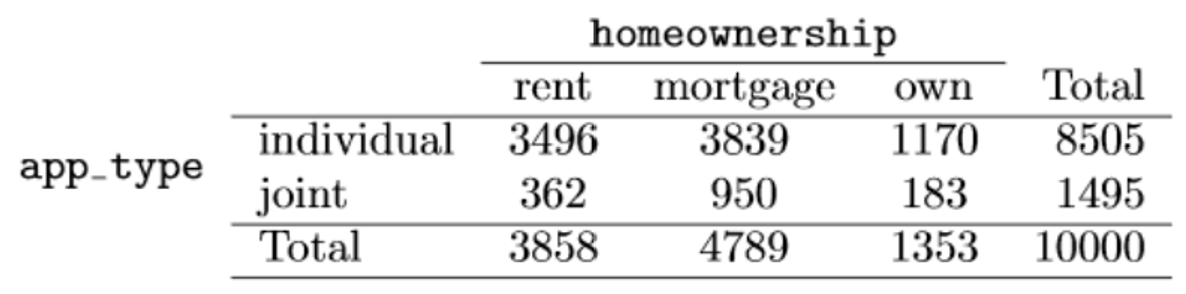
\includegraphics[scale=0.7]{images/contingency.png}
\end{center}

Question of interest: Does there appear to be a relationship between loan application type and homeownership status? We can start to answer this question by examining row proportions:

\begin{itemize}

\item \% of all applicants who rent: \vspace{20pt}

\item \% of individual applicants who rent: \vspace{20pt}

\item \% of joint applicants who rent: \vspace{40pt}
\end{itemize}

{\bf Bar Plots}


\begin{center}
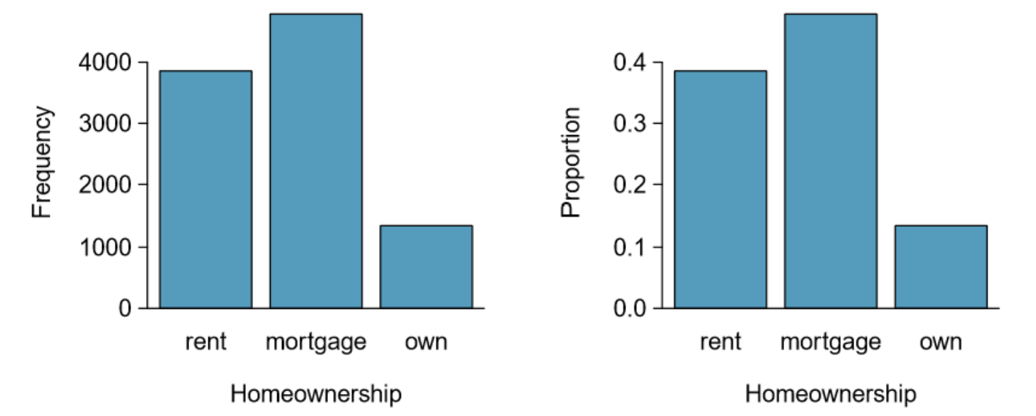
\includegraphics[scale=0.8]{images/barplot.png}
\end{center}

Differences between bar plots and histograms?

\newpage

{\bf Pie Charts}

\begin{center}
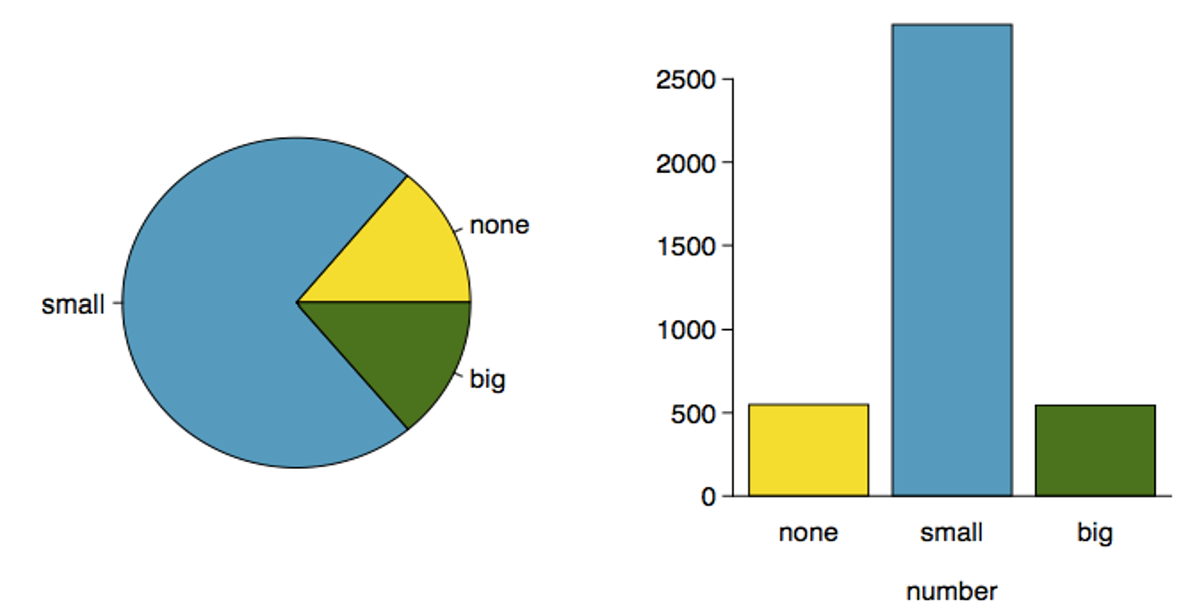
\includegraphics[scale=0.7]{images/pie.png}
\end{center}

{\bf Side-by-Side Plots}

\begin{center}
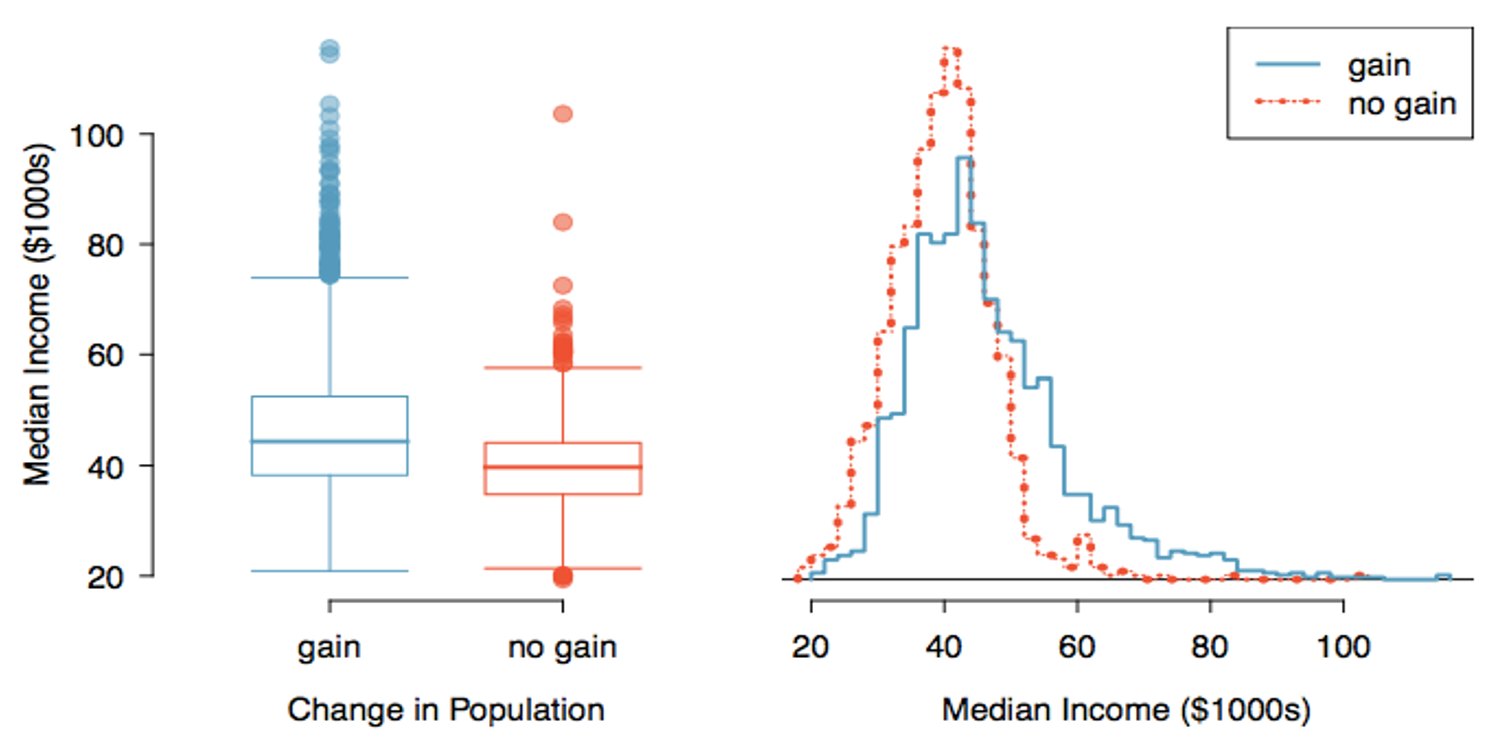
\includegraphics[scale=0.8]{images/sidebyside.png}
\end{center}

\label{totalpag}
\end{document}